%%%%%%%%%%%%%%%%%%%%%%%%%%%%%%%%%%%%%%%%%%%%%%%%%%%%%%%%%%%%%%%%%%%%%%
% How to use writeLaTeX: 
%
% You edit the source code here on the left, and the preview on the
% right shows you the result within a few seconds.
%
% Bookmark this page and share the URL with your co-authors. They can
% edit at the same time!
%
% You can upload figures, bibliographies, custom classes and
% styles using the files menu.
%
%%%%%%%%%%%%%%%%%%%%%%%%%%%%%%%%%%%%%%%%%%%%%%%%%%%%%%%%%%%%%%%%%%%%%%

\documentclass[12pt]{article}

\usepackage{sbc-template}

\usepackage{graphicx,url}
\usepackage{hyperref}

%\usepackage[brazil]{babel}   
\usepackage[utf8]{inputenc}  

     
\sloppy

\title{Relatório: Trabalho Prático 2\\ Soluções para problemas difíceis}

\author{ Marcos Paulo F. de Souza\inst{1} }


\address{
  Departamento de Ciência da Computação\\
  Universidade Federal de Minas Gerais (UFMG) -- Belo Horizonte, MG -- Brazil
  \email{marcos.ferreira@dcc.ufmg.br}
}

\begin{document} 

\maketitle

\begin{abstract}
  This work aimed to investigate and compare the performance of different algorithms for solving the traveling salesman problem. Three algorithms were implemented and analyzed: Branch and Bound, Twice-around-the-tree, and Christofides. The results obtained demonstrate that the Branch and Bound algorithm, although exact, exhibits a high computational cost. On the other hand, the probabilistic algorithms Twice-around-the-tree and Christofides proved to be more efficient in terms of execution time, providing approximate solutions much faster. The Christofides algorithm exhibited better performance in terms of solution quality, and the Twice-around-the-tree algorithm stood out for its speed.
\end{abstract}
     
\begin{resumo} 
  Este trabalho teve como objetivo investigar e comparar o desempenho de diferentes algoritmos para resolver o problema do caixeiro viajante. Foram implementados e analisados três algoritmos: Branch and Bound, Twice-around-the-tree e Christofides. Os resultados obtidos demonstram que o algoritmo Branch and Bound, embora seja exato, apresenta um custo computacional elevado. Por outro lado, os algoritmos probabilísticos Twice-around-the-tree e Christofides se mostraram mais eficientes em termos de tempo de execução, fornecendo soluções aproximadas muito mais rapidamente. O algoritmo Christofides apresentou um melhor desempenho em termos de qualidade da solução, e o algoritmo Twice-around-the-tree se destacou pela sua rapidez.
\end{resumo}


\section{Introdução}

Esse trabalho apresenta uma análise comparativa de diferentes algoritmos que resolvem o problema do caixeiro viajante. O problema do caixeiro viajante é um problema de otimização NP-difícil, ou seja, encontrar uma solução exata é muito custoso computacionalmente, podendo levar milhares de anos a depender do tamanho da instância do problema. 

Foram implementados e comparados três algoritmos representativos que são o Branch and Bound, Twice-around-the-tree e Christofides. O algoritmo Branch and Bound é um algoritmo exato baseado em busca em árvore, enquanto os algoritmos Twice-around-the-tree e Christofides são probabilísticos e fornecem soluções aproximadas.

O trabalho está organizado da seguinte forma: na primeira seção, é apresentado o problema do caixeiro viajante e a relevância de sua solução. Em seguida, são descritos os algoritmos implementados, detalhando suas principais características e a lógica implementada. Na sequência, são apresentados os resultados obtidos com os testes, comparando o desempenho dos algoritmos em termos de tempo de execução e qualidade das soluções. Por fim, são discutidas as principais conclusões resultantes do trabalho.

\section{Conceitos Básicos}

O problema do caixeiro viajante foi apresentado por Anany Levitin em seu livro chamado "Introduction to The Design and Analysis of Algorithms". A sucinta definição do problema trazida foi a de encontrar a menor rota possível passando por N cidades, apenas uma vez por cidade, e depois retornando para a cidade de origem. Esse problema é classificado como  NP-Difícil, portanto ele pode ser resolvido em tempo polinomial por uma máquina de Turing não determinística. Isso significa que os computadores atuais não são capazes de encontrar uma solução para esse problema em tempo hábil. Por isso, são precisos algoritmos mais complexos para encontrar uma solução mais rapidamente. Para este trabalho serão implementados três algoritmos que resolvem esse problema. O primeiro algoritmo é o Branch and Bound, o segundo é o algoritmo aproximativo Twice-around-the-tree e o terceiro é o algoritmo aproximativo Christofides. Toda a definição das implementações foram retiradas do livro "Introduction to The Design and Analysis of Algorithms".

\section{Implementação}

A implementação dos três algoritmos foi feita em um mesmo arquivo na linguagem de programação python. Foram usadas as bibliotecas math e networkx para a implementação dos algoritmos. As bibliotecas os e timeout\_decorator foram usados durante os testes para automatizar a execução dos testes e limitar o tempo de execução de cada algoritmo respectivamente. Já as bibliotecas matplotlib e pandas foram usadas para gerar as tabelas e os resultados para serem analisados.

Os três algoritmos terão as suas implementações detalhadas a seguir:

\subsection{Branch and Bound}

Para a implementação desse algoritmo a estrutura de dados Graph disponibilizada pela biblioteca networkx foi utilizada, além de alguns métodos auxiliares que foram implementados à parte e estão contidos no mesmo arquivo dos demais algoritmos.

Para ser um algoritmo Branch and Bound é preciso ter o cálculo de uma estimativa que seja realista e próxima ao valor ótimo. O cálculo da estimativa que foi implementado foi o mesmo descrito por Levitin no livro "Introduction to The Design and Analysis of Algorithms". Em resumo, a estimativa é a soma das duas arestas de menor custo de todos os nós do grafo divido por dois. Quando uma aresta é introduzida na possível solução ela é considerada como uma das menores arestas dos nós que ela liga. E isso garante que a estimativa seja realista.

A árvore de soluções possíveis é armazenada como uma fila de prioridades onde a solução que possui a menor estimativa tem a maior prioridade. Ou seja, para avançar na árvore de soluções possíveis é usada a busca em largura, escolhendo sempre a solução com menor estimativa e não a que esteja mais profunda na árvore.

\subsection{Twice-around-the-tree}

Para a implementação desse algoritmo a estrutura de dados Graph e os algoritmos minimum\_spanning\_tree e dfs\_preorder\_nodes que são disponibilizados pela biblioteca networkx foram utilizados.

A implementação desse algoritmo foi feita como é descrita no livro "Introduction to The Design and Analysis of Algorithms". São três passos a serem feitos, o primeiro é calcular a árvore geradora mínima para o grafo da instância do problema, o segundo passo é definir a lista de vértices da árvores geradora mínima a partir de visitação preorder dos vértices e o terceiro e último passo é retirar da lista de vértices os que estão repetidos, encontrando o ciclo hamiltoniano do grafo, que é a solução para o problema.

\subsection{Christofides}

Para a implementação desse algoritmo a estrutura de dados Graph e os algoritmos minimum\_spanning\_tree, min\_weight\_matching e eulerian\_circuit que são disponibilizados pela biblioteca networkx foram utilizados, além de um método auxiliar que foi implementado a parte e está contido no mesmo arquivo dos demais algoritmos.

A implementação desse algoritmo foi feita como é descrita no livro "Introduction to The Design and Analysis of Algorithms". Essa implementação é semelhante a do algoritmo Twice-around-the-tree porém com algumas alterações. Primeiro é necessário encontrar a árvore geradora mínima e depois gerar uma lista de nós da árvore geradora mínima que possuem grau ímpar. Dentro do subgrafo induzido pelos nós de grau ímpar é encontrado o matching perfeito de peso mínimo. Com isso será criado um grafo auxiliar que adiciona na árvore geradora mínima todas as arestas do matching perfeito de peso mínimo. Nesse grafo auxiliar é calculado o circuito euleriano e com a lista de vértices do circuito euleriano basta retirar os vértices repetidos e encontraremos o circuito hamiltoniano que é a solução para o problema.

\section{Testes}

Os algoritmos implementados foram testados usando as intâncias contidas no site \href{http://comopt.ifi.uni-heidelberg.de/software/TSPLIB95/tsp/}{http://comopt.ifi.uni-heidelberg.de/software/TSPLIB95/tsp/}. Dentre todas as instâncias disponíveis apenas as euclidianas com 2 dimensões foram usadas, totalizando 77 instâncias. Desses testes, existem 5 que possuem mais do que 7000 cidades e não puderam ser executados, pois o computador utilizado não possui poder computacional o suficiente para terminar esses testes, que causaram travamentos e a reinicialização do computador. Portanto, foram executadas 72 instâncias do problema, e cada instância foi executada uma vez em cada algoritmo implementado. Cada algoritmo possui um limite de 30 minutos para encontrar uma solução, caso o algoritmo não tivesse parado de executar nesse limite de tempo ele era interrompido e o resultado ficava como NA (não-disponível).

\subsection{Resultados}

O resultado dos testes (Figura \ref{fig:fig1}) mostram como o aumento do número de cidades teve uma influência no aumento do tempo gasto executando os algoritmos. O algoritmo de Branch and Bound não possui variação, pois não conseguiu terminar nenhuma das instâncias antes do limite do tempo. Podemos ver que o algoritmo mais afetado pelo aumento do número de cidades foi o algoritmo de Christofides, chegando a não concluir a execução de uma instância.

\begin{figure}[ht]
\centering
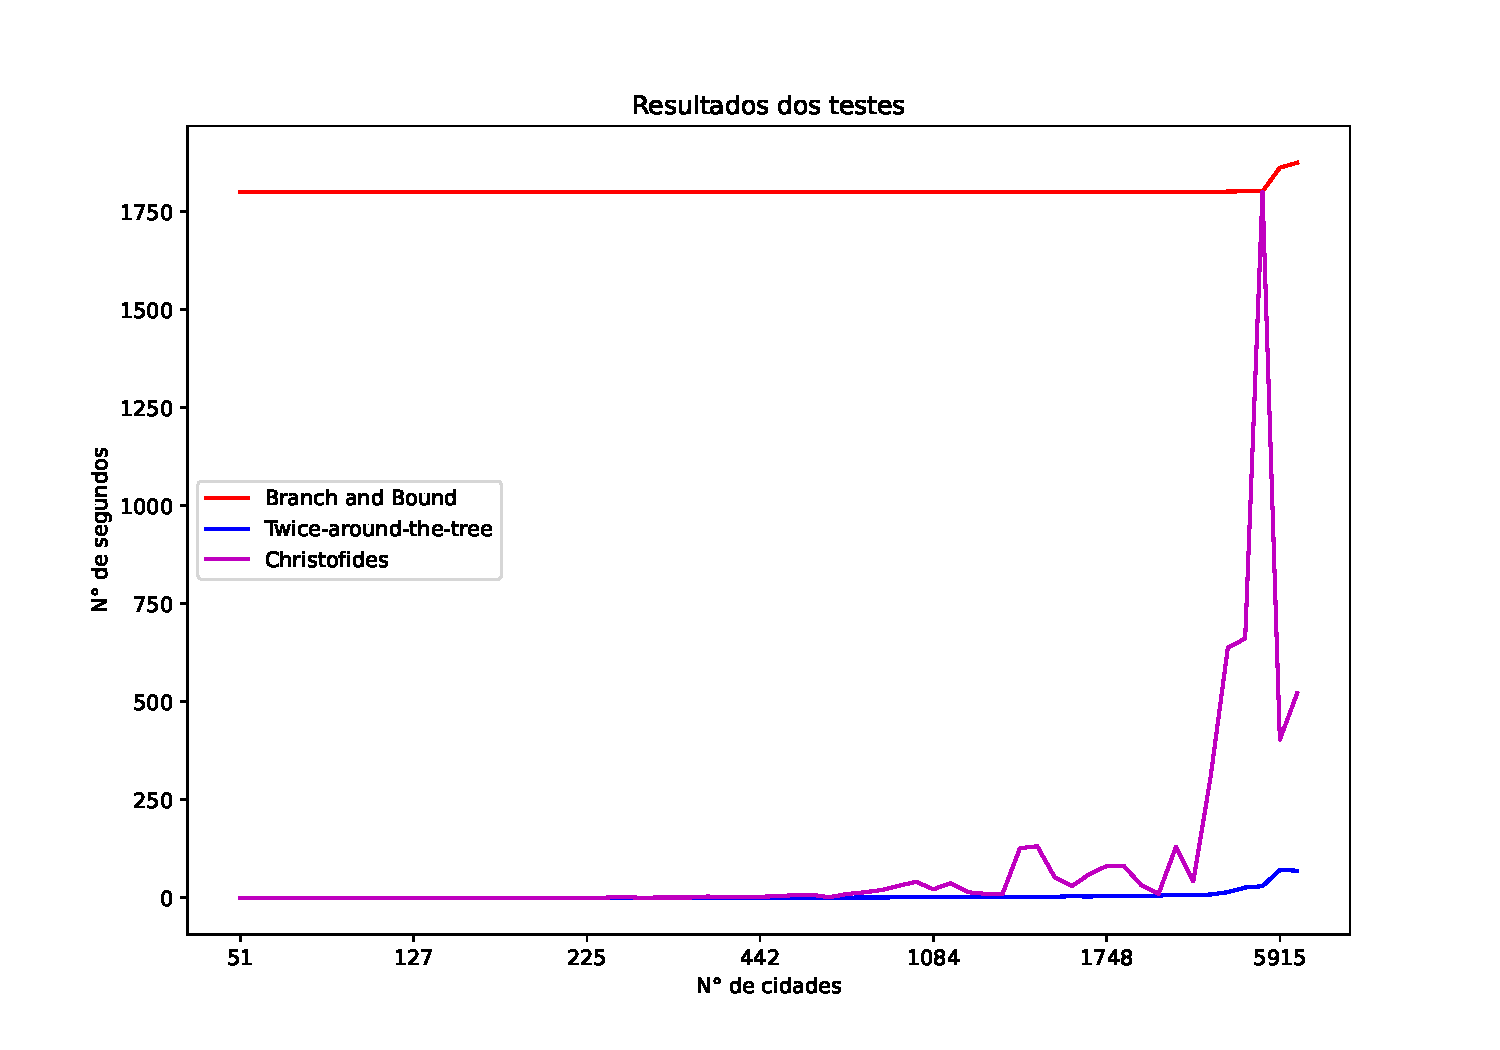
\includegraphics[width=.8\textwidth]{../Figura1.pdf}
\caption{Tabela com os resultados de todos algoritmos}
\label{fig:fig1}
\end{figure}

O algoritmo Branch and Bound não encontrou a solução de nenhum dos testes devido a sua grande complexidade de execução, que nos piores casos pode ser equivalente a uma solução ingênua de força bruta.

O algoritmo Twice-around-the-tree encontrou uma solução para todas as instâncias em tempo inferior a 90 segundos (Figura \ref{fig:fig2}). Mostrando ser uma excelente opção quando é preciso de uma solução rápida e que não precisa ser exata para o problema do caixeiro viajante.

\begin{figure}[ht]
\centering
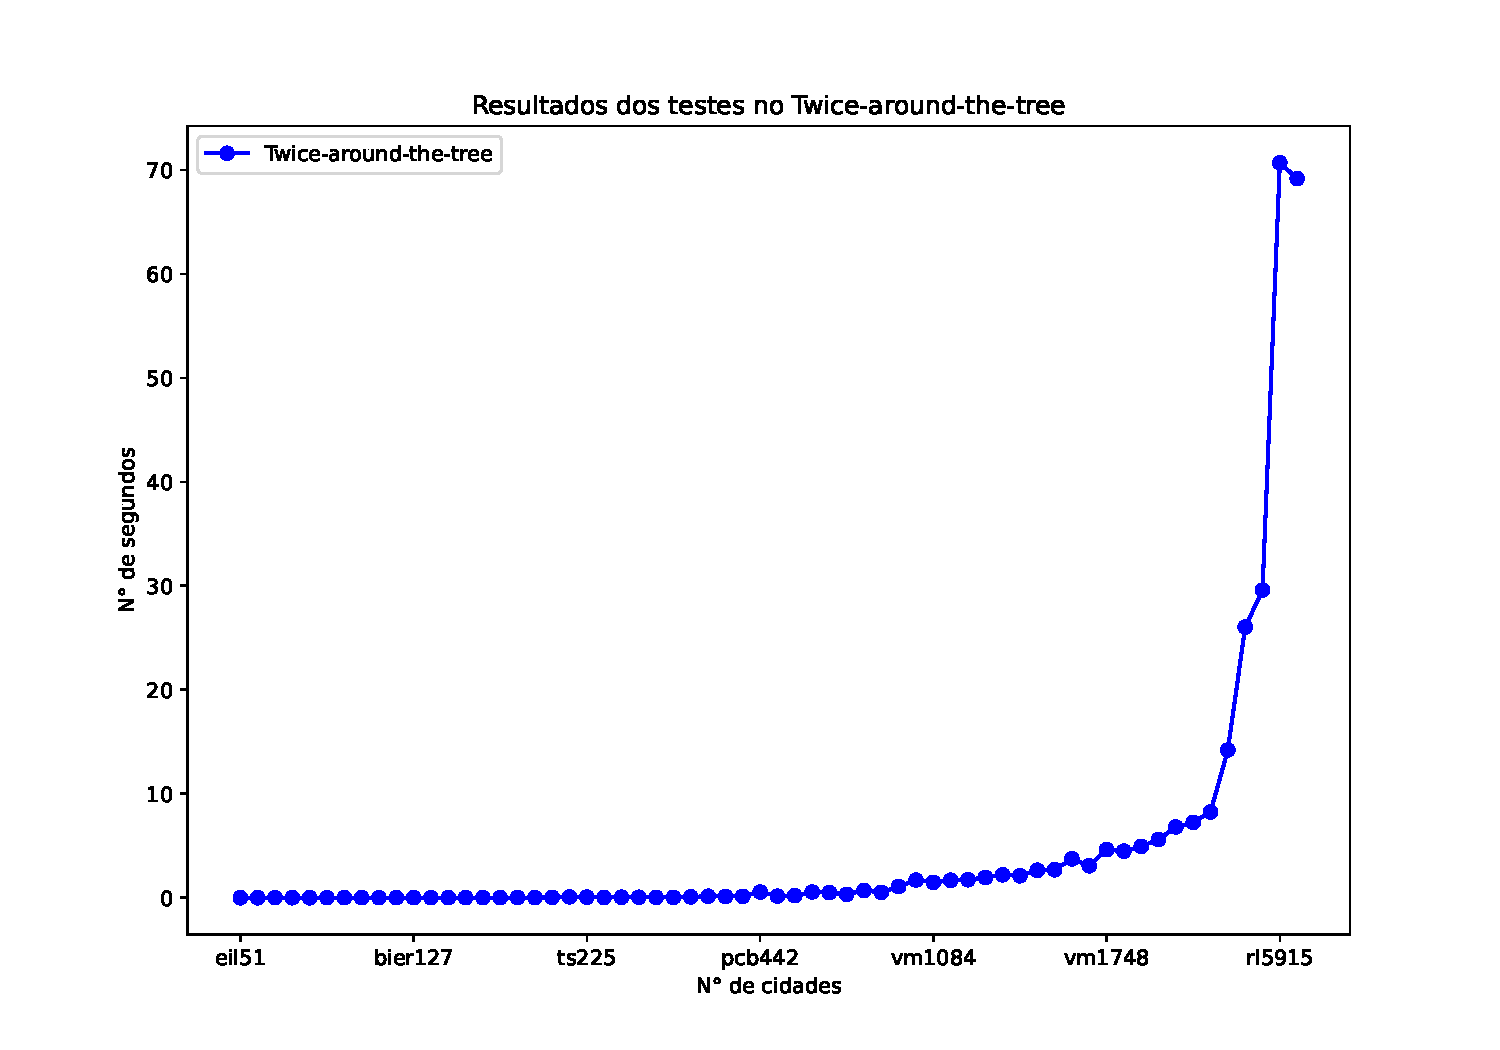
\includegraphics[width=.6\textwidth]{../Figura2.pdf}
\caption{Tabela com os resultados do Twice-around-the-tree}
\label{fig:fig2}
\end{figure}

O algoritmo Christofides encontrou a solução para 71 das 72 instâncias que foram testadas no tempo definido. Ele possui uma maior variação do tempo de execução, porém ele traz soluções mais próximas da ótima.

\begin{figure}[ht]
\centering
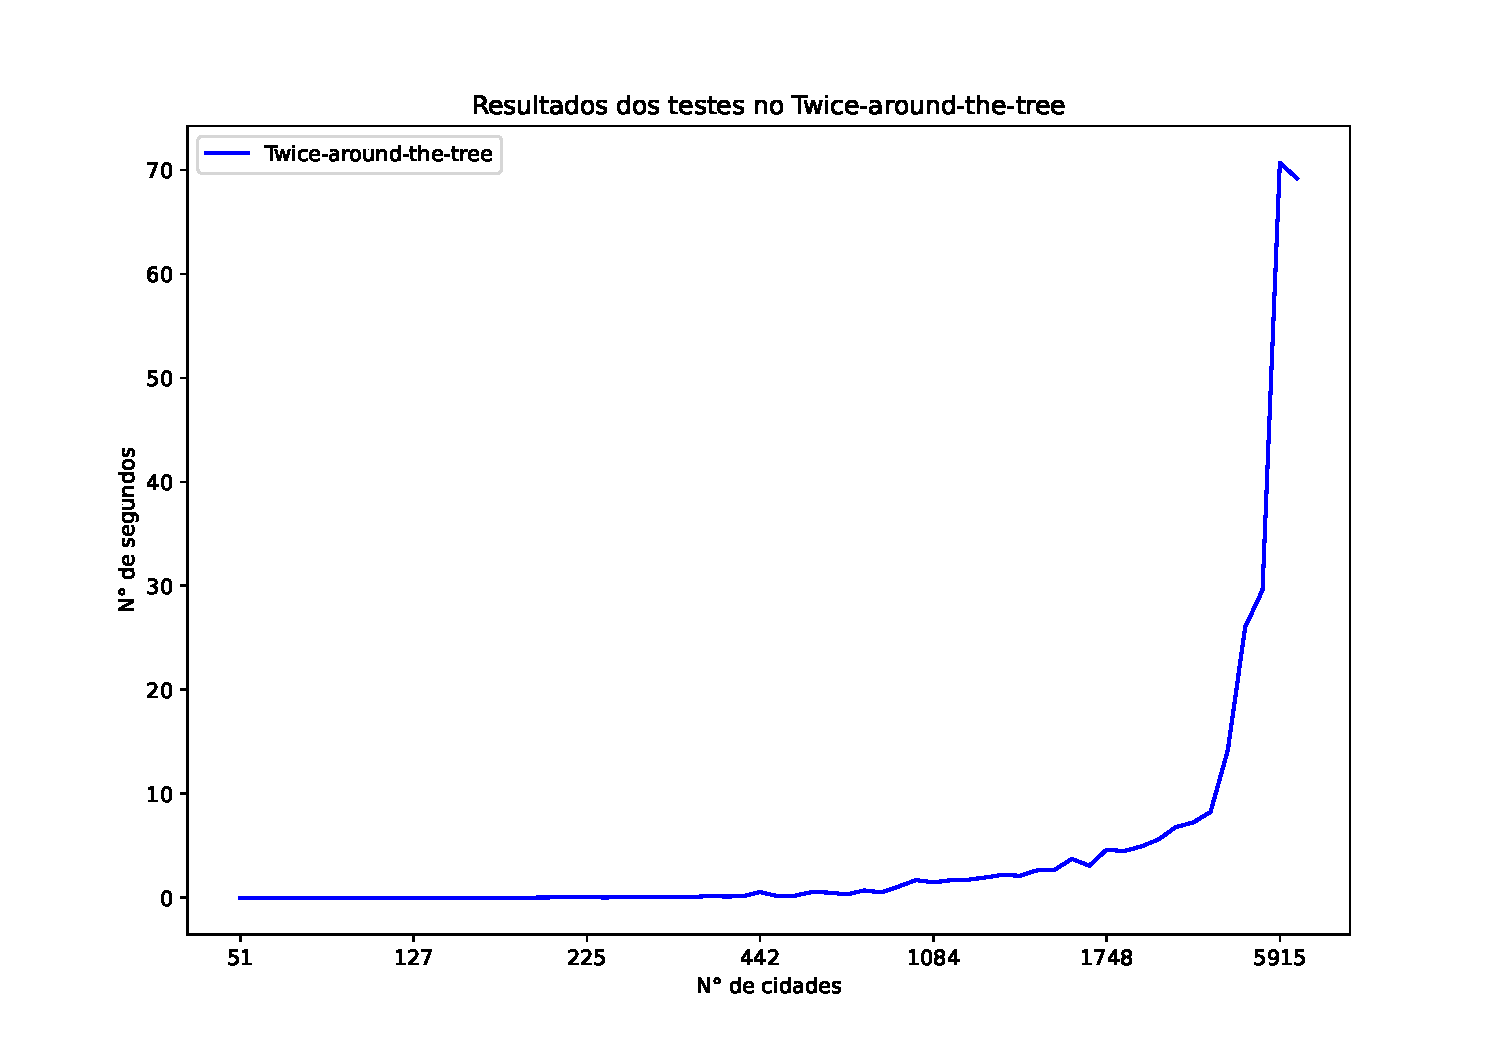
\includegraphics[width=.8\textwidth]{../Figura3.pdf}
\caption{Tabela com a comparação do resultado dos testes}
\label{fig:fig3}
\end{figure}

Comparando os resultados obtidos nos testes com os melhores resultados (Figura \ref{fig:fig3}) disponibilizados pelo \href{http://comopt.ifi.uni-heidelberg.de/software/TSPLIB95/tsp/}{site}, podemos observar que os algoritmos encontram soluções proximas as melhores. O algoritmo Twice-around-the-tree encontrou as soluções mais distantes das melhores, isso é o esperado já que a taxa de aproximação desse algoritmo é de no máximo duas vezes a solução ótima. O algoritmo de Christofides, que encontrou as soluções mais próximas às melhores, tem o resultado esperado já que posuui uma taxa de aproximação de no máximo um em meio da solução ótima. O custo do algoritmo de Christofides para encontrar uma solução mais próxima da melhor é ter um maior custo computacional e por isso ele possui um maior tempo de execução que o algoritmo Twice-around-the-tree. 

\section{Conclusão}

Neste trabalho, foram implementados e comparados três algoritmos que resolvem o problema do caixeiro viajante e eles são: Branch and Bound, Twice-around-the-tree e Christofides. Os resultados obtidos demonstram que o algoritmo Branch and Bound, apesar de sua exatidão, apresenta um custo computacional tão grande que nenhuma das instâncias testadas teve uma solução encontrada dentro do tempo limite estabelecido. Por outro lado, os algoritmos probabilísticos Twice-around-the-tree e Christofides apresentaram um desempenho superior em termos de tempo de execução, fornecendo soluções aproximadas relativamente rápido.

O algoritmo de Christofides se mostrou mais preciso, porém com um custo computacional maior. O algoritmo Twice-around-the-tree se destacou pela sua rapidez, sendo uma opção para aplicações que exigem soluções rápidas, mesmo que não sejam ótimas.

Com esses resultados é possível compreender as características e limitações de cada algoritmo, auxiliando na escolha da melhor abordagem para diferentes cenários práticos.

\begin{thebibliography}{1}

\bibitem{christofides} 
    \textit{Introduction to the design \& analysis of algorithms}. Disponível em: \url{https://homel.vsb.cz/~fai0013/Kniha_Algoritmy.pdf}. Acesso em: 16 jan. 2025.

\end{thebibliography}

\end{document}
